\documentclass[11pt,a4paper]{report}
\usepackage[textwidth=37em,vmargin=30mm]{geometry}
\usepackage{calc,xunicode,amsmath,amssymb,paralist,enumitem,tabu,booktabs,datetime2,xeCJK,xeCJKfntef,listings}
\usepackage{tocloft,fancyhdr,tcolorbox,xcolor,graphicx,eso-pic,xltxtra,xelatexemoji}

\newcommand{\envyear}[0]{2025}
\newcommand{\envdatestr}[0]{2025-06-05}
\newcommand{\envfinaldir}[0]{webdb/2025/20250605/final}

\usepackage[hidelinks]{hyperref}
\hypersetup{
    colorlinks=false,
    pdfpagemode=FullScreen,
    pdftitle={Web Digest - \envdatestr}
}

\setlength{\cftbeforechapskip}{10pt}
\renewcommand{\cftchapfont}{\rmfamily\bfseries\large\raggedright}
\setlength{\cftbeforesecskip}{2pt}
\renewcommand{\cftsecfont}{\sffamily\small\raggedright}

\setdefaultleftmargin{2em}{2em}{1em}{1em}{1em}{1em}

\usepackage{xeCJK,xeCJKfntef}
\xeCJKsetup{PunctStyle=plain,RubberPunctSkip=false,CJKglue=\strut\hskip 0pt plus 0.1em minus 0.05em,CJKecglue=\strut\hskip 0.22em plus 0.2em}
\XeTeXlinebreaklocale "zh"
\XeTeXlinebreakskip = 0pt


\setmainfont{Brygada 1918}
\setromanfont{Brygada 1918}
\setsansfont{IBM Plex Sans}
\setmonofont{JetBrains Mono NL}
\setCJKmainfont{Noto Serif CJK SC}
\setCJKromanfont{Noto Serif CJK SC}
\setCJKsansfont{Noto Sans CJK SC}
\setCJKmonofont{Noto Sans CJK SC}

\setlength{\parindent}{0pt}
\setlength{\parskip}{8pt}
\linespread{1.15}

\lstset{
	basicstyle=\ttfamily\footnotesize,
	numbersep=5pt,
	backgroundcolor=\color{black!5},
	showspaces=false,
	showstringspaces=false,
	showtabs=false,
	tabsize=2,
	captionpos=b,
	breaklines=true,
	breakatwhitespace=true,
	breakautoindent=true,
	linewidth=\textwidth
}






\newcommand{\coverpic}[2]{
    % argv: itemurl, authorname
    Cover photo by #2~~(\href{#1}{#1})
}
\newcommand{\makeheader}[0]{
    \begin{titlepage}
        % \newgeometry{hmargin=15mm,tmargin=21mm,bmargin=12mm}
        \begin{center}
            
            \rmfamily\scshape
            \fontspec{BaskervilleF}
            \fontspec{Old Standard}
            \fontsize{59pt}{70pt}\selectfont
            WEB\hfill DIGEST
            
            \vfill
            % \vskip 30pt
            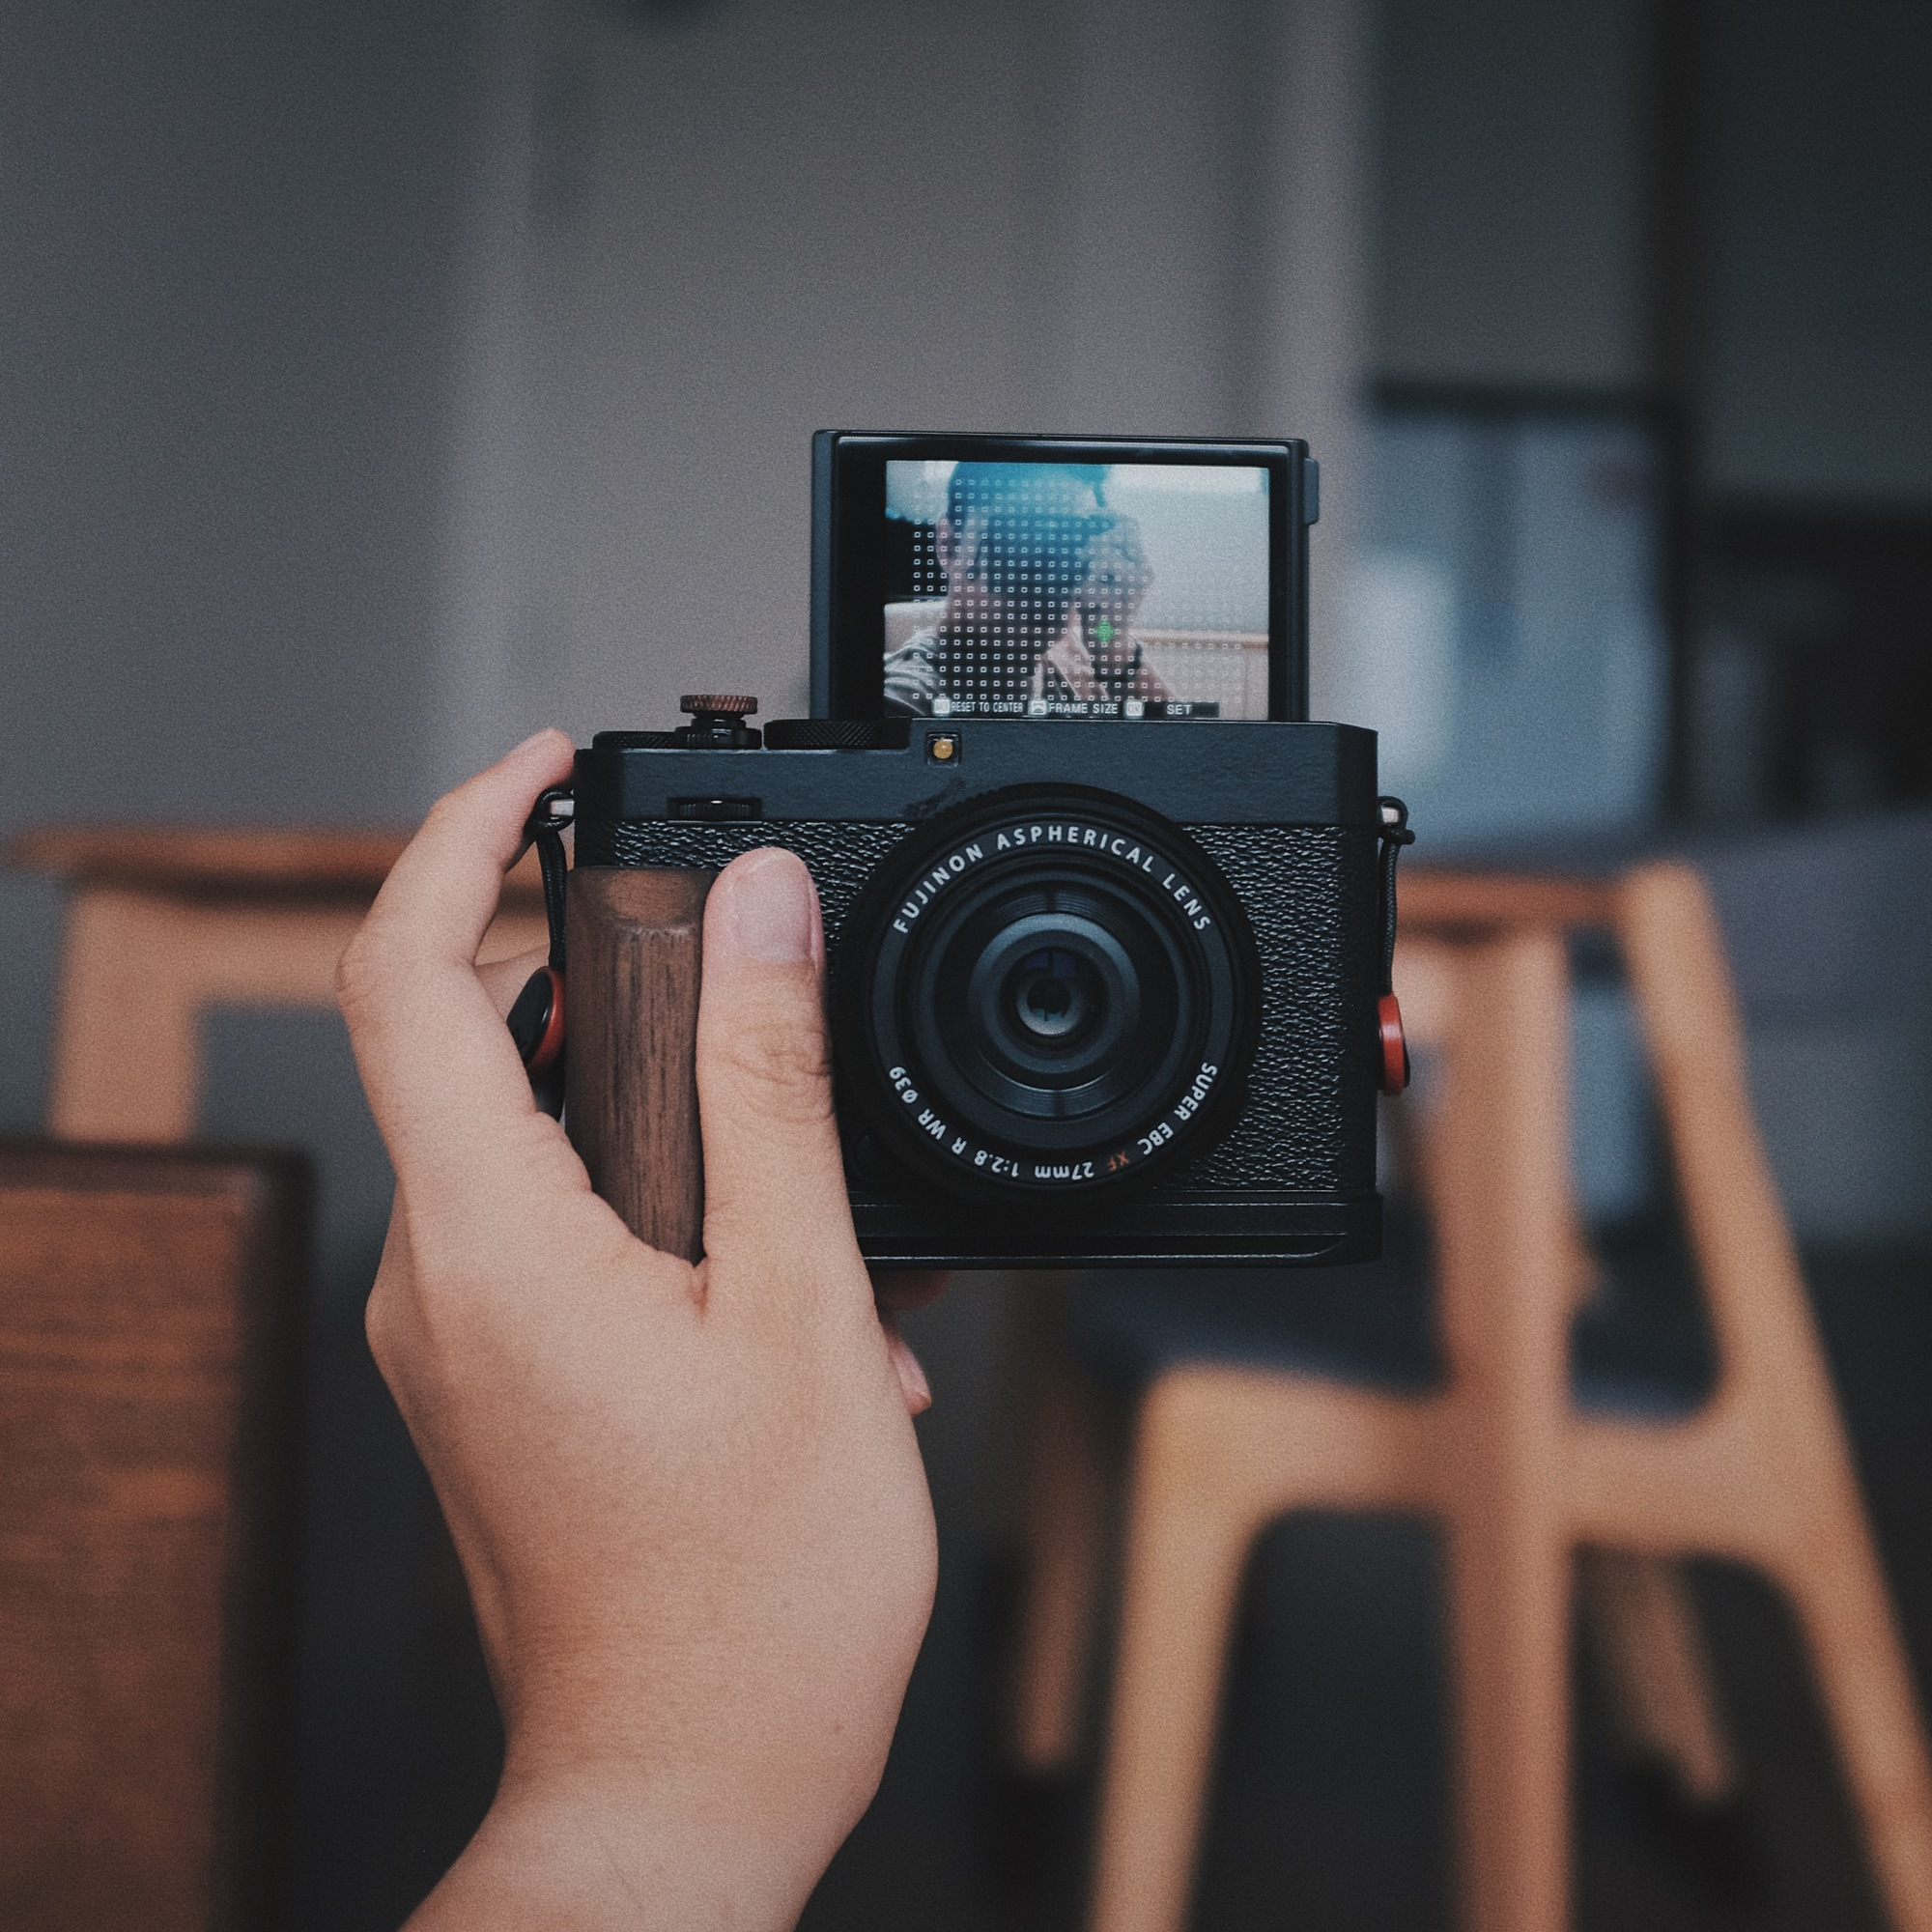
\includegraphics[width=\linewidth]{\envfinaldir/coverpic-prod.jpg}\par
            % \vskip 30pt
            \vfill

            \normalsize\rmfamily\scshape
            \copyright{} The Web Digest Project \hfill\large \envdatestr
        \end{center}
    \end{titlepage}
    % \restoregeometry
}
\newcommand{\simplehref}[1]{%
    \textcolor{blue!80!green}{\href{#1}{#1}}%
}
\renewcommand{\contentsname}{\center\Huge\sffamily\bfseries Contents\par\vskip 20pt}
\newcounter{ipartcounter}
\setcounter{ipartcounter}{0}
\newcommand{\ipart}[1]{
    % \vskip 20pt
    \clearpage
    \stepcounter{ipartcounter}
    \phantomsection
    \addcontentsline{toc}{chapter}{#1}
    % \begin{center}
    %     \Huge
    %     \sffamily\bfseries
    %     #1
    % \end{center}
    % \vskip 20pt plus 7pt
}
\newcounter{ichaptercounter}
\setcounter{ichaptercounter}{0}
\newcommand{\ichapter}[1]{
    % \vskip 20pt
    \clearpage
    \stepcounter{ichaptercounter}
    \phantomsection
    \addcontentsline{toc}{section}{\numberline{\arabic{ichaptercounter}}#1}
    \begin{center}
        \Huge
        \sffamily\bfseries
        #1
    \end{center}
    \vskip 20pt plus 7pt
}
\newcommand{\entrytitlefont}[1]{\subsection*{\raggedright\Large\sffamily\bfseries#1}}
\newcommand{\entryitemGeneric}[2]{
    % argv: title, url
    \parbox{\linewidth}{
        \entrytitlefont{#1}\par\vskip 5pt
        \footnotesize\ttfamily\mdseries
        \simplehref{#2}
    }\vskip 11pt plus 11pt minus 1pt
}
\newcommand{\entryitemGithub}[3]{
    % argv: title, url, desc
    \parbox{\linewidth}{
        \entrytitlefont{#1}\par\vskip 5pt
        \footnotesize\ttfamily\mdseries
        \simplehref{#2}\par\vskip 5pt
        \small\rmfamily\mdseries#3
    }\vskip 11pt plus 11pt minus 1pt
}
\newcommand{\entryitemAp}[3]{
    % argv: title, url, desc
    \parbox{\linewidth}{
        \entrytitlefont{#1}\par\vskip 5pt
        \footnotesize\ttfamily\mdseries
        \simplehref{#2}\par\vskip 5pt
        \small\rmfamily\mdseries#3
    }\vskip 11pt plus 11pt minus 1pt
}
\newcommand{\entryitemHackernews}[3]{
    % argv: title, hnurl, rawurl
    % \parbox{\linewidth}{
    %     \entrytitlefont{#1}\par\vskip 5pt
    %     \footnotesize\ttfamily\mdseries
    %     \simplehref{#3}\par
    %     \textcolor{black!50}{\href{#2}{#2}}
    % }\vskip 11pt plus 11pt minus 1pt
    \begin{minipage}{\linewidth}
            \entrytitlefont{#1}\par\vskip 5pt
            \footnotesize\ttfamily\mdseries
            \simplehref{#3}\par
            \textcolor{black!50}{\href{#2}{#2}}
    \end{minipage}\par\vskip 11pt plus 11pt minus 1pt
}







\begin{document}

\makeheader

\tableofcontents\clearpage




\ipart{Developers}
\ichapter{Hacker News}
\entryitemTwoLinks{After court order, OpenAI is now preserving all ChatGPT user logs}{https://news.ycombinator.com/item?id=44185913}{https://mastodon.laurenweinstein.org/@lauren/114627064774788581}

\entryitemTwoLinks{Cursor 1.0}{https://news.ycombinator.com/item?id=44185256}{https://www.cursor.com/en/changelog/1-0}

\entryitemTwoLinks{Autonomous drone defeats human champions in racing first}{https://news.ycombinator.com/item?id=44184900}{https://www.tudelft.nl/en/2025/lr/autonomous-drone-from-tu-delft-defeats-human-champions-in-historic-racing-first}

\entryitemTwoLinks{Redesigned Swift.org is now live}{https://news.ycombinator.com/item?id=44184542}{https://swift.org/}

\entryitemTwoLinks{Curtis Yarvin's Plot Against America}{https://news.ycombinator.com/item?id=44184305}{https://www.newyorker.com/magazine/2025/06/09/curtis-yarvin-profile}

\entryitemTwoLinks{Apple Notes Expected to Gain Markdown Support in iOS 26}{https://news.ycombinator.com/item?id=44183923}{https://www.macrumors.com/2025/06/04/apple-notes-rumored-markdown-support-ios-26/}

\entryitemTwoLinks{A proposal to restrict sites from accessing a users' local network}{https://news.ycombinator.com/item?id=44183799}{https://github.com/explainers-by-googlers/local-network-access}

\entryitemTwoLinks{The iPhone 15 Pro's Depth Maps}{https://news.ycombinator.com/item?id=44183591}{https://tech.marksblogg.com/apple-iphone-15-pro-depth-map-heic.html}

\entryitemTwoLinks{Mistral Code}{https://news.ycombinator.com/item?id=44183515}{https://mistral.ai/products/mistral-code}

\entryitemTwoLinks{We are no longer a serious country}{https://news.ycombinator.com/item?id=44182634}{https://paulkrugman.substack.com/p/we-are-no-longer-a-serious-country}

\entryitemTwoLinks{VC money is fueling a global boom in worker surveillance tech}{https://news.ycombinator.com/item?id=44182582}{https://restofworld.org/2025/employee-surveillance-software-vc-funding/}

\entryitemTwoLinks{IRS Direct File on GitHub}{https://news.ycombinator.com/item?id=44182356}{https://chrisgiven.com/2025/05/direct-file-on-github/}

\entryitemTwoLinks{Meta found 'covertly tracking' Android users through Instagram and Facebook}{https://news.ycombinator.com/item?id=44182204}{https://news.sky.com/story/meta-found-covertly-tracking-android-users-through-instagram-and-facebook-13379083}

\entryitemTwoLinks{The Prompt Engineering Playbook for Programmers}{https://news.ycombinator.com/item?id=44182188}{https://addyo.substack.com/p/the-prompt-engineering-playbook-for}

\entryitemTwoLinks{FFmpeg merges WebRTC support}{https://news.ycombinator.com/item?id=44182186}{https://git.ffmpeg.org/gitweb/ffmpeg.git/commit/167e343bbe75515a80db8ee72ffa0c607c944a00}

\entryitemTwoLinks{A practical guide to building agents [pdf]}{https://news.ycombinator.com/item?id=44181700}{https://cdn.openai.com/business-guides-and-resources/a-practical-guide-to-building-agents.pdf}

\entryitemTwoLinks{The Right to Repair Is Law in Washington State}{https://news.ycombinator.com/item?id=44181421}{https://www.eff.org/deeplinks/2025/06/right-repair-law-washington-state}

\entryitemTwoLinks{"AI Will Replace All the Jobs " Is Just Tech Execs Doing Marketing}{https://news.ycombinator.com/item?id=44181172}{https://sparktoro.com/blog/ai-will-replace-all-the-jobs-is-just-tech-execs-doing-marketing/}

\entryitemTwoLinks{The Sky's the limit: AI automation on Mac}{https://news.ycombinator.com/item?id=44179691}{https://taoofmac.com/space/blog/2025/06/03/2155}

\entryitemTwoLinks{Just how bad are we at treating age-related diseases?}{https://news.ycombinator.com/item?id=44179329}{https://www.ladanuzhna.xyz/writing/just-how-bad-are-we-at-treating-age-related-diseases}\ichapter{Dribbble}
\entryitemGeneric{\hskip 0pt{}Aquasan}{https://dribbble.com/shots/26100535-Aquasan}

\entryitemGeneric{\hskip 0pt{}Eagle}{https://dribbble.com/shots/26099428-Eagle}

\entryitemGeneric{\hskip 0pt{}Mnp Technologies - Logo Design}{https://dribbble.com/shots/26092034-Mnp-Technologies-Logo-Design}

\entryitemGeneric{\hskip 0pt{}Singular Logo Concept (Unused)}{https://dribbble.com/shots/26091755-Singular-Logo-Concept-Unused}

\entryitemGeneric{\hskip 0pt{}Cre8tera // Website}{https://dribbble.com/shots/26091009-Cre8tera-Website}

\entryitemGeneric{\hskip 0pt{}Cool Pool Logo Design - Letter C Monogram}{https://dribbble.com/shots/26091401-Cool-Pool-Logo-Design-Letter-C-Monogram}

\entryitemGeneric{\hskip 0pt{}Gorilla + Bar Chart Logo}{https://dribbble.com/shots/26092670-Gorilla-Bar-Chart-Logo}

\entryitemGeneric{\hskip 0pt{}zeero logo design}{https://dribbble.com/shots/26087342-zeero-logo-design}

\entryitemGeneric{\hskip 0pt{}Create email inbox composition}{https://dribbble.com/shots/26083118-Create-email-inbox-composition}

\entryitemGeneric{\hskip 0pt{}Shori Brand}{https://dribbble.com/shots/26088139-Shori-Brand}

\entryitemGeneric{\hskip 0pt{}Roaring Bear}{https://dribbble.com/shots/26087788-Roaring-Bear}

\entryitemGeneric{\hskip 0pt{}Eagle}{https://dribbble.com/shots/26085536-Eagle}

\entryitemGeneric{\hskip 0pt{}Hand-drawn illustration pack}{https://dribbble.com/shots/26084735-Hand-drawn-illustration-pack}

\entryitemGeneric{\hskip 0pt{}Dog Mascot Various Poses}{https://dribbble.com/shots/26087977-Dog-Mascot-Various-Poses}

\entryitemGeneric{\hskip 0pt{}Branding Concept for Europe}{https://dribbble.com/shots/26087652-Branding-Concept-for-Europe}

\entryitemGeneric{\hskip 0pt{}B2B Dashboard \& Web App UI UX Design for Carbon Solutions}{https://dribbble.com/shots/26076624-B2B-Dashboard-Web-App-UI-UX-Design-for-Carbon-Solutions}

\entryitemGeneric{\hskip 0pt{}Patriot Logo Design (Unused for Sale)}{https://dribbble.com/shots/26081047-Patriot-Logo-Design-Unused-for-Sale}

\entryitemGeneric{\hskip 0pt{}Heliopoint}{https://dribbble.com/shots/26081987-Heliopoint}

\entryitemGeneric{\hskip 0pt{}Apple}{https://dribbble.com/shots/26084067-Apple}

\entryitemGeneric{\hskip 0pt{}Illustration}{https://dribbble.com/shots/26083223-Illustration}

\entryitemGeneric{\hskip 0pt{}Europe Logo Animation}{https://dribbble.com/shots/26082596-Europe-Logo-Animation}

\entryitemGeneric{\hskip 0pt{}Arc Logo}{https://dribbble.com/shots/26083648-Arc-Logo}

\entryitemGeneric{\hskip 0pt{}Heyo Turns 2!}{https://dribbble.com/shots/26078572-Heyo-Turns-2}

\entryitemGeneric{\hskip 0pt{}Fox Brand Mascot}{https://dribbble.com/shots/26077954-Fox-Brand-Mascot}


\ipart{Developers~~~~(zh-Hans)}
\ichapter{Solidot}
\entryitemGeneric{\hskip 0pt{}日本 2024 年新生儿数首次跌破 70 万}{https://www.solidot.org/story?sid=81466}

\entryitemGeneric{\hskip 0pt{}AI 创业公司被发现其聊天机器人是 700 名印度员工}{https://www.solidot.org/story?sid=81465}

\entryitemGeneric{\hskip 0pt{}OpenAI 董事会短暂解雇 CEO Sam Altman 的故事被搬上银幕}{https://www.solidot.org/story?sid=81464}

\entryitemGeneric{\hskip 0pt{}乌克兰使用开源软件对俄罗斯后方机场轰炸机发动无人机攻击}{https://www.solidot.org/story?sid=81461}

\entryitemGeneric{\hskip 0pt{}印度便利店应用 KiranaPro 被删库}{https://www.solidot.org/story?sid=81460}

\entryitemGeneric{\hskip 0pt{}研究确定背包问题计算复杂性下限}{https://www.solidot.org/story?sid=81459}

\entryitemGeneric{\hskip 0pt{}神秘告密者公开勒索软件组织关键成员身份}{https://www.solidot.org/story?sid=81458}

\entryitemGeneric{\hskip 0pt{}报告称 AI 的普及和增长``史无前例''}{https://www.solidot.org/story?sid=81457}

\entryitemGeneric{\hskip 0pt{}仙女座和银河系未必会相撞}{https://www.solidot.org/story?sid=81456}

\entryitemGeneric{\hskip 0pt{}锻炼能显著降低结肠癌的复发和死亡风险}{https://www.solidot.org/story?sid=81455}

\entryitemGeneric{\hskip 0pt{}微软对 Windows 11 设备强制统一 USB-C 功能}{https://www.solidot.org/story?sid=81454}

\entryitemGeneric{\hskip 0pt{}Stack Overflow 的衰落始于其声誉系统}{https://www.solidot.org/story?sid=81453}

\entryitemGeneric{\hskip 0pt{}中国出现假装上班的新商业模式}{https://www.solidot.org/story?sid=81452}

\entryitemGeneric{\hskip 0pt{}微软 Google 等将统一国家支持的黑客组织的绰号}{https://www.solidot.org/story?sid=81451}

\entryitemGeneric{\hskip 0pt{}美国部分 incel 选择躺平}{https://www.solidot.org/story?sid=81450}

\entryitemGeneric{\hskip 0pt{}朝鲜智能手机会自动替换禁词每 5 分钟截屏}{https://www.solidot.org/story?sid=81449}

\entryitemGeneric{\hskip 0pt{}我国科学家构建 300 公里级量子直接通信网络}{https://www.solidot.org/story?sid=81448}

\entryitemGeneric{\hskip 0pt{}M8.2 级太阳耀斑引发 G4 级地磁风暴}{https://www.solidot.org/story?sid=81447}

\entryitemGeneric{\hskip 0pt{}美国的加密货币战略储备规模有多大}{https://www.solidot.org/story?sid=81446}\ichapter{V2EX}
\entryitemGeneric{\hskip 0pt{}[问与答] 兄弟们,留不住钱怎么办?}{https://www.v2ex.com/t/1136426}

\entryitemGeneric{\hskip 0pt{}[VXNA] 申请收录:白宦成的博客}{https://www.v2ex.com/t/1136425}

\entryitemGeneric{\hskip 0pt{}[分享发现] 我发现了微信顶着被骂被喷也要把服务号折叠到一起的原因}{https://www.v2ex.com/t/1136424}

\entryitemGeneric{\hskip 0pt{}[程序员] 请问大佬们平时写代码要写几遍啊?}{https://www.v2ex.com/t/1136423}

\entryitemGeneric{\hskip 0pt{}[音乐] 你们听蔡徐坤的《deadman》了吗?}{https://www.v2ex.com/t/1136422}

\entryitemGeneric{\hskip 0pt{}[全球工单系统] 大厂的傲慢 - 腾讯云注销一个账户,咋就这么难?}{https://www.v2ex.com/t/1136421}

\entryitemGeneric{\hskip 0pt{}[OpenAI] 最好的购买官方 gpt plus 方法?}{https://www.v2ex.com/t/1136420}

\entryitemGeneric{\hskip 0pt{}[分享发现] Gemini Pro 思考速度有明显提升}{https://www.v2ex.com/t/1136418}

\entryitemGeneric{\hskip 0pt{}[问与答] 给家里院子安装几个监控什么品牌好}{https://www.v2ex.com/t/1136417}

\entryitemGeneric{\hskip 0pt{}[问与答] Windows 有什么启动器 可以 记录搜索的文件 或者 打开的文件夹,从而再次快速定位的软件吗?}{https://www.v2ex.com/t/1136416}

\entryitemGeneric{\hskip 0pt{}[宽带症候群] 软路由选购疑问}{https://www.v2ex.com/t/1136415}

\entryitemGeneric{\hskip 0pt{}[酷工作] 成都(3 天公司 2 天在家): Junior/Intermediate Developer,短期项目, 1000-1200/天}{https://www.v2ex.com/t/1136413}

\entryitemGeneric{\hskip 0pt{}[OpenWrt] 请教一下 openwrt 中使用 open 克拉斯如何做 dns 服务器}{https://www.v2ex.com/t/1136412}

\entryitemGeneric{\hskip 0pt{}[宽带症候群] 求助 本地网络对 未响应端口进行了``伪装成功连接''处理}{https://www.v2ex.com/t/1136411}

\entryitemGeneric{\hskip 0pt{}[分享创造] 史上最简 ``临时文件'' 服务}{https://www.v2ex.com/t/1136410}

\entryitemGeneric{\hskip 0pt{}[问与答] 618 耳机选购求助}{https://www.v2ex.com/t/1136408}

\entryitemGeneric{\hskip 0pt{}[生活] 楼下每天打麻将到凌晨一点,但不是我正下方,要不要冲下去沟通?}{https://www.v2ex.com/t/1136407}

\entryitemGeneric{\hskip 0pt{}[旅行] 法意瑞路线 2.0,继续求建议}{https://www.v2ex.com/t/1136405}

\entryitemGeneric{\hskip 0pt{}[酷工作] [招聘] [北京] 客户端(RN)、全栈(Node)、AI Agent 工程师}{https://www.v2ex.com/t/1136404}

\entryitemGeneric{\hskip 0pt{}[路由器] 小米 AX3000 的无线问题}{https://www.v2ex.com/t/1136403}

\entryitemGeneric{\hskip 0pt{}[Windows] 求助: 神舟战神笔记本 刷成安卓 TV 后,刷不回 Win 了}{https://www.v2ex.com/t/1136402}

\entryitemGeneric{\hskip 0pt{}[分享创造] PicSharp:开源、多平台、小而美的图片压缩工具,支持本地和 TinyPNG 压缩}{https://www.v2ex.com/t/1136401}

\entryitemGeneric{\hskip 0pt{}[酷工作] [招聘][远程][币安] 前端/后端/测开/DevOps/PM 至少 3 年以上经验 目前有大量 HC 欢迎投递}{https://www.v2ex.com/t/1136400}

\entryitemGeneric{\hskip 0pt{}[远程工作] [伦敦 AI 初创企业] 高级 React 工程师}{https://www.v2ex.com/t/1136399}

\entryitemGeneric{\hskip 0pt{}[程序员] minio 后台移除了 admin 相关的操作权限}{https://www.v2ex.com/t/1136395}

\entryitemGeneric{\hskip 0pt{}[问与答] 被抖音杀熟了怎么办?}{https://www.v2ex.com/t/1136394}

\entryitemGeneric{\hskip 0pt{}[问与答] 你们都在用什么型号的笔记本}{https://www.v2ex.com/t/1136393}

\entryitemGeneric{\hskip 0pt{}[生活] 看教育相关贴有感,回忆一下我的学生时代}{https://www.v2ex.com/t/1136392}

\entryitemGeneric{\hskip 0pt{}[VPS] 某些特殊业务,服务器该怎么选?}{https://www.v2ex.com/t/1136391}

\entryitemGeneric{\hskip 0pt{}[Windows] 为什么今天 windows 11 的商店打不开了}{https://www.v2ex.com/t/1136390}

\entryitemGeneric{\hskip 0pt{}[问与答] 关于 BBR+Moonlight 串流卡顿的问题求教}{https://www.v2ex.com/t/1136389}

\entryitemGeneric{\hskip 0pt{}[游戏] lol 手游双人竞技场符文刷新次数规则}{https://www.v2ex.com/t/1136388}

\entryitemGeneric{\hskip 0pt{}[MacBook Pro] better touch tool 玩了两天,还是没玩会.}{https://www.v2ex.com/t/1136387}

\entryitemGeneric{\hskip 0pt{}[分享创造] 分享一个自己开发的脚手架,基于 DDD 领域设计的}{https://www.v2ex.com/t/1136386}

\entryitemGeneric{\hskip 0pt{}[iPhone] 一个小工具解决系统数据过大问题}{https://www.v2ex.com/t/1136385}

\entryitemGeneric{\hskip 0pt{}[Notion] 我有点难以理解 notion 子页的逻辑}{https://www.v2ex.com/t/1136383}

\entryitemGeneric{\hskip 0pt{}[创业组队] 有一个点子,但是缺一个有分布式系统架构经验的程序员合伙人一起完成一款产品,不知道有没有人有兴趣或者可以提点建议}{https://www.v2ex.com/t/1136382}

\entryitemGeneric{\hskip 0pt{}[Node.js] 做了一个函数式、带类型、超顺手的微型事件库,已发布到 npm}{https://www.v2ex.com/t/1136381}

\entryitemGeneric{\hskip 0pt{}[生活] 咨询:二线城市买地盖房问题}{https://www.v2ex.com/t/1136380}

\entryitemGeneric{\hskip 0pt{}[郑州] 郑州-招前端、产品、设计岗,纯自研产品-扁平弹性双休}{https://www.v2ex.com/t/1136379}

\entryitemGeneric{\hskip 0pt{}[分享创造] 实在没有 Idea, 用 Cursor 写了一个美国身份信息生成器,欢迎大家来体验一下}{https://www.v2ex.com/t/1136377}

\entryitemGeneric{\hskip 0pt{}[教育] 求推荐一个无线打印机,孩子作业用的}{https://www.v2ex.com/t/1136376}

\entryitemGeneric{\hskip 0pt{}[问与答] 今天大家一起来弄清楚甲骨文升级号扩展区域收费问题}{https://www.v2ex.com/t/1136375}

\entryitemGeneric{\hskip 0pt{}[MacBook Pro] 有必要剩国补换电脑吗?}{https://www.v2ex.com/t/1136374}

\entryitemGeneric{\hskip 0pt{}[分享创造] 一款期望键盘用户用着安心的焦点导航库, naviix,输入元素的定位和尺寸,输出每个元素的十字方向相邻元素}{https://www.v2ex.com/t/1136372}

\entryitemGeneric{\hskip 0pt{}[职场话题] 有没有创业的家伙?你们每天工作多少小时?}{https://www.v2ex.com/t/1136371}

\entryitemGeneric{\hskip 0pt{}[问与答] 大家有觉得在某些极限场景下流量卡比正常的手机卡网速要慢吗}{https://www.v2ex.com/t/1136370}

\entryitemGeneric{\hskip 0pt{}[程序员] MoonBit 推出面向 markdown 编程功能,配合 CI 可以保证代码不过时}{https://www.v2ex.com/t/1136369}

\entryitemGeneric{\hskip 0pt{}[摄影] 重生之我在草原拍牛马}{https://www.v2ex.com/t/1136368}

\entryitemGeneric{\hskip 0pt{}[问与答] 求罗技 master3s 替代方案}{https://www.v2ex.com/t/1136367}


\ipart{Generic News}
\ichapter{AP News}
\entryitemWithDescription{\hskip 0pt{}FanDuel bans bettor over heckling incident with Olympic champion sprinter Gabby Thomas}{https://apnews.com/article/d226103292fdf6c019f0c71435e9745e}{}

\entryitemWithDescription{\hskip 0pt{}Ex-White House press secretary Karine Jean-Pierre left Democratic Party, publisher of her book says}{https://apnews.com/article/fbb44b9eb3bb56f6ab8ef02bd7ffa042}{}

\entryitemWithDescription{\hskip 0pt{}Dilly Dally the sea turtle returns to the ocean after flipper amputation}{https://apnews.com/article/3310f37f8901e539453c22ca40dabc00}{}

\entryitemWithDescription{\hskip 0pt{}Hegseth orders the name of gay rights activist Harvey Milk scrubbed from Navy ship}{https://apnews.com/article/d6cda5df15ee5bc066092d54c591c6f2}{}

\entryitemWithDescription{\hskip 0pt{}Reddit sues AI company Anthropic for allegedly `scraping' user comments to train chatbot Claude}{https://apnews.com/article/f5ea042beb253a3f05a091e70531692d}{}

\entryitemWithDescription{\hskip 0pt{}A long-running experiment finds a tiny particle is still acting weird}{https://apnews.com/article/cb123cd20bfd8141dbf75de62804b32b}{}

\entryitemWithDescription{\hskip 0pt{}Woman who denies mushroom murders of her in-laws accepts that she served them death caps for lunch}{https://apnews.com/article/00ea28021943fe4a56d2a3b30ad26598}{}

\entryitemWithDescription{\hskip 0pt{}What made Mount Etna's latest eruption so rare}{https://apnews.com/article/1adafac765158138817a2c4319ce1468}{}

\entryitemWithDescription{\hskip 0pt{}Northern lights could be visible again in some US states after weekend solar storms}{https://apnews.com/article/915a2364b24679c63a07066f55c53ffa}{}

\entryitemWithDescription{\hskip 0pt{}Eagles' Saquon Barkley announced as Madden NFL 26 cover athlete}{https://apnews.com/article/3b0254fa10fb8df98e91562be76d8d5c}{}

\entryitemWithDescription{\hskip 0pt{}Bills QB Josh Allen and actor Hailee Steinfeld marry in Southern California}{https://apnews.com/article/7d152f7f490a3d8ee28d6031bf02b3a0}{}

\entryitemWithDescription{\hskip 0pt{}And with that, an era ends: `Thanks for watching us. It's the NBA on TNT'}{https://apnews.com/article/8d11e74bf32e77de886add0225f108ef}{}

\entryitemWithDescription{\hskip 0pt{}The NBA Finals are set: It'll be Thunder vs. Pacers, starting Thursday night}{https://apnews.com/article/fcb0ef3120847d1d6f515fc5fe5bf04a}{}\ichapter{Reuters}
\entryitemWithDescription{\hskip 0pt{}Pro-Russian, anti-Israeli hackers pose biggest cybercrime threats in Germany}{https://www.reuters.com/sustainability/boards-policy-regulation/pro-russian-anti-israeli-hackers-pose-biggest-cybercrime-threats-germany-2025-06-03/}{Cybercrime in Germany rose to a record level last year, driven by hacker attacks from pro-Russian and anti-Israeli groups, the BKA Federal Crime Office reported on Tuesday as the government said it would boost countermeasures to combat...}

\entryitemWithDescription{\hskip 0pt{}Polish parliament speaker says confidence vote should be next week}{https://www.reuters.com/world/europe/polish-parliament-speaker-says-confidence-vote-should-be-next-week-2025-06-03/}{Polish Parliament Speaker Szymon Holownia proposed on Tuesday that a vote of confidence in the government should take place in a week at an additional session of...}

\entryitemWithDescription{\hskip 0pt{}Philippines keeps Cabinet mostly unchanged after 'bold reset' call}{https://www.reuters.com/world/asia-pacific/philippines-keeps-cabinet-mostly-unchanged-after-bold-reset-call-2025-06-03/}{Philippine President Ferdinand Marcos Jr has retained the majority of his Cabinet ministers, two weeks after requesting their resignations in what he called a bold reset of his administration, his executive secretary said on...}

\entryitemWithDescription{\hskip 0pt{}Germany's Merz says court ruling will not stop migration crackdown}{https://www.reuters.com/world/europe/germanys-merz-says-court-ruling-will-not-stop-migration-crackdown-2025-06-03/}{Chancellor Friedrich Merz said on Tuesday a court ruling that German authorities acted unlawfully when border police expelled three Somali asylum seekers could restrict his government\textquotesingle s migration crackdown but would not...}

\entryitemWithDescription{\hskip 0pt{}UN convoy attacked on the way to Sudan's al-Fashir, UNICEF says}{https://www.reuters.com/world/africa/un-convoy-attacked-way-sudans-al-fashir-unicef-says-2025-06-03/}{A U.N. convoy delivering food into Sudan\textquotesingle s al-Fashir in North Darfur came under attack overnight, a spokesperson for the U.N. children\textquotesingle s agency told Reuters on Tuesday, adding that initial reports...}

\entryitemWithDescription{\hskip 0pt{}More than 4 million refugees have fled Sudan since war began, UN says}{https://www.reuters.com/world/africa/more-than-4-million-refugees-have-fled-sudan-since-war-began-un-says-2025-06-03/}{The number of people who have fled Sudan since the beginning of the war has surpassed 4 million, a spokesperson for the U.N. refugee agency said on...}

\entryitemWithDescription{\hskip 0pt{}Ukraine president's chief of staff in US for talks on defence support}{https://www.reuters.com/world/europe/ukraine-presidents-chief-staff-us-talks-defence-support-2025-06-03/}{A Ukrainian government delegation arrived in Washington on Tuesday to discuss military support and sanctions against Russia, a day after Kyiv and Moscow held their second round of peace...}

\entryitemWithDescription{\hskip 0pt{}Soft-focus interview positions Bardella as leader-in-waiting of France's far-right}{https://www.reuters.com/world/europe/soft-focus-interview-positions-bardella-leader-in-waiting-frances-far-right-2025-06-03/}{Jordan Bardella, the 29-year-old wunderkind of France\textquotesingle s far right National Rally (RN), says he grew up wanting to be Superman, or James Bond. These days, he dreams of marrying a tall brunette with a strong...}

\entryitemWithDescription{\hskip 0pt{}Russian attack on Ukrainian city Sumy kills two people}{https://www.reuters.com/world/europe/russian-attack-ukrainian-city-sumy-kills-two-people-2025-06-03/}{A Russian attack on Ukraine\textquotesingle s northeastern city of Sumy killed two people and injured at least seven more, including four children, local prosecutors said in a statement on...}

\entryitemWithDescription{\hskip 0pt{}Medvedev says Russia seeks victory, not compromise, in talks with Ukraine}{https://www.reuters.com/world/europe/medvedev-says-russia-seeks-victory-not-compromise-talks-with-ukraine-2025-06-03/}{Senior Russian security official Dmitry Medvedev said on Tuesday that the point of holding peace talks with Ukraine was to ensure a swift and complete Russian...}

\entryitemWithDescription{\hskip 0pt{}Dutch government on brink of collapse after Wilders' far-right party quits}{https://www.reuters.com/world/europe/dutch-far-right-leader-wilders-quits-government-coalition-nos-2025-06-03/}{Dutch far-right leader Geert Wilders\textquotesingle{} PVV party left the governing coalition on Tuesday, in a move that is set to topple the right wing government and likely lead to new...}

\entryitemWithDescription{\hskip 0pt{}Myanmar junta says extends temporary ceasefire to June 30}{https://www.reuters.com/world/asia-pacific/myanmar-junta-says-extends-temporary-ceasefire-june-30-2025-06-03/}{Myanmar\textquotesingle s junta said it has extended a temporary ceasefire to June to support reconstruction and relief efforts following a massive earthquake in late March that killed at least 3,700 people and devastated parts of the...}

\entryitemWithDescription{\hskip 0pt{}At least 27 Palestinians killed near Gaza aid site, medics say}{https://www.reuters.com/world/middle-east/least-24-palestinians-killed-near-gaza-aid-site-medics-say-2025-06-03/}{At least 27 Palestinians were killed and dozens wounded by Israeli fire near a food distribution site in the southern Gaza Strip, in the third day of chaos and bloodshed to affect the aid...}






\clearpage
\leavevmode\vfill
\footnotesize

Copyright \copyright{} 2023-2025 Neruthes and other contributors.

This document is published with CC BY-NC-ND 4.0 license.

The entries listed in this newsletter may be copyrighted by their respective creators.

This newsletter is generated by the Web Digest project.

The newsletters are also delivered via Telegram channel \CJKunderline{\href{https://t.me/webdigestchannel}{https://t.me/webdigestchannel}}.\\
RSS feed is available at \CJKunderline{\href{https://webdigest.pages.dev/rss.xml}{https://webdigest.pages.dev/rss.xml}}.

This newsletter is available in PDF at
\CJKunderline{\href{https://webdigest.pages.dev/}{https://webdigest.pages.dev/}}.

The source code being used to generate this newsletter is available at\\
\CJKunderline{\href{https://github.com/neruthes/webdigest}{https://github.com/neruthes/webdigest}}.

This newsletter is also available in
\CJKunderline{\href{http://webdigest.pages.dev/readhtml/\envyear/WebDigest-20250605.html}{HTML}} and
\CJKunderline{\href{https://github.com/neruthes/webdigest/blob/master/markdown/\envyear/WebDigest-20250605.md}{Markdown}}.


\coverpic{https://unsplash.com/photos/two-fashionable-dogs-look-up-on-a-yellow-background-Me-iF3302T8}{Karsten Winegeart}


\end{document}
